\subsection{Photoresistor}\label{sub:photoresistor}
A photoresistor is a variable resistor, which reacts to light, meaning that, the resistance the resistor exerts falls as the light intensity rises. The photoresistor, used in this project, has the part number VT90N2 and the data sheet can be found in \cite{photoresistor_sheet}. As can be seen in the data sheet, this resistor has a typical resistance of 24k $\Omega$ when at 10 lux (a lux scale can be found at \cite{lux_scale}) and 500k $\Omega$ in at 0 lux. The response time is the time between two consecutive readings. Response time, when the light intensity is higher than approximately 11 lux is under 0.1 seconds. When the light intensity is lower than approximately 11 lux, the response time can increase to at most 0.8 seconds. At 0 \degree C, there can be up to about 13\% variance in the reported resistance. At 40 \degree C, the variance can be up to 20\%. While this is a high variance, the variance normalises to 0\% at around 25 \degree C. The photoresistor is sensitive to light outside the visible spectrum. It is below 18\% sensitive to some wavelengths below 400 nm, which means ultraviolet light could affect readings. It is below 5\% sensitive to light above 800 nm, which means that infrared light can be considered a negligible interference.

Because the resistor is too sensitive for the purpose of this project, a pull-down resistor is added to the circuit\cite{pulldown_resistor}. A pull-down resistor lowers the base value, this means that we can detect higher levels of light. An example setup can be seen in \cref{fig:arduino_photoresistor_wiring}. For the experiments two identical setups were used, with varying pull-down resistors strength.

\begin{figure}[htbp]
  \centering
  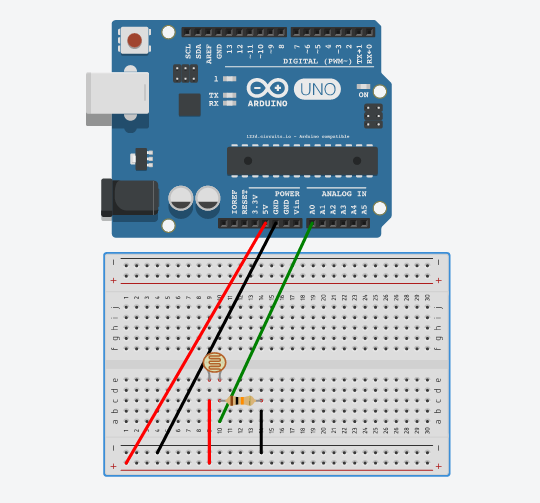
\includegraphics[width=\textwidth]{Implementation/hardware/PhotoSensorTests/Images/photoresistor_setup.png}
  \caption[Photoresistor]{The figure depicts wiring for a photoresistor with a pull-down resistor.}\label{fig:arduino_photoresistor_wiring}
\end{figure}

\subsubsection{Sampling Input Data}
To reduce noise on the signal of the sensor, the sensor is probed 10 times. The average of these readings is the result.
